\documentclass[UTF8]{ctexbeamer}

\usetheme{Pittsburgh}
\usefonttheme[onlymath]{serif}

\usepackage{subfig}
\usepackage{multirow}
\usepackage{xcolor,colortbl}
\usepackage{listings}
\usepackage{amsmath}

% Solarized colors
\definecolor{sbase03}{HTML}{002B36}
\definecolor{sbase02}{HTML}{073642}
\definecolor{sbase01}{HTML}{586E75}
\definecolor{sbase00}{HTML}{657B83}
\definecolor{sbase0}{HTML}{839496}
\definecolor{sbase1}{HTML}{93A1A1}
\definecolor{sbase2}{HTML}{EEE8D5}
\definecolor{sbase3}{HTML}{FDF6E3}
\definecolor{syellow}{HTML}{B58900}
\definecolor{sorange}{HTML}{CB4B16}
\definecolor{sred}{HTML}{DC322F}
\definecolor{smagenta}{HTML}{D33682}
\definecolor{sviolet}{HTML}{6C71C4}
\definecolor{sblue}{HTML}{268BD2}
\definecolor{scyan}{HTML}{2AA198}
\definecolor{sgreen}{HTML}{859900}

\lstset{
    % How/what to match
    sensitive=true,
    % Border (above and below)
    frame=lines,
    % Extra margin on line (align with paragraph)
    xleftmargin=\parindent,
    % Put extra space under caption
    belowcaptionskip=1\baselineskip,
    % Colors
    backgroundcolor=\color{sbase3},
    basicstyle=\color{sbase00}\ttfamily,
    keywordstyle=\color{scyan},
    commentstyle=\color{sbase1},
    stringstyle=\color{sblue},
    numberstyle=\color{sviolet},
    identifierstyle=\color{sbase00},
    % Break long lines into multiple lines?
    breaklines=true,
    % Show a character for spaces?
    showstringspaces=false,
    tabsize=2
}


% Title
\title{第8章 图论建模}
\author{韩建伟}
\institute{
  信息学院\\
  \texttt{mm@hanjianwei.com}
}
\date{2017/12/01}

\begin{document}

% Title page
\begin{frame}[plain]
  \titlepage{}
\end{frame}

\begin{frame}{垒球队教练的问题}
  如何挑出一个11人的首发阵容?

  \begin{table}
    \centering
    \begin{tabular}{c|c|c|c|c|c|c|c}
      \hline
      Al & Bo & Che & Doug & Ella & Fay & Gene & Hal\\
      \hline
      2,8 & 1,5,7 & 2,3 & 1,4,5,6,7 & 3,8 & 10,11 & 3,8,11 & 2,4,9\\
      \hline
      Ian & John & Kit & Leo & Moe & Ned & Paul & \\
      \hline
      8,9,10 & 1,5,6,7 & 8,9 & 3,9,11 & 1,4,6,7 && 9,10 &\\
      \hline
    \end{tabular}
  \end{table}

  如果Hal不能打二垒呢?

  \begin{table}
    \centering
    \begin{tabular}{c|c|c|c|c|c|c|c}
      \hline
      Al & Bo & Che & Doug & Ella & Fay & Gene & Hal\\
      \hline
      2,8 & 1,5,7 & 2,3 & 1,4,5,6,7 & 3,8 & 10,11 & 3,8,11 & 2,9\\
      \hline
      Ian & John & Kit & Leo & Moe & Ned & Paul & \\
      \hline
      8,9,10 & 1,5,6,7 & 8,9 & 3,9,11 & 1,4,6,7 && 9,10 &\\
      \hline
    \end{tabular}
  \end{table}
  
\end{frame}

\begin{frame}{哥尼斯堡七桥问题}

  \begin{block}{欧拉问题}
    \begin{itemize}
    \item 从该市的某处出发,走过每座桥而且只走一次,最后回到原地可能吗?
    \item 给定一个图,在什么样的条件下有可能找到一条封闭的散步路线,能走过它的每一条边,而且只走一次?
    \end{itemize}
  \end{block}

  \begin{figure}
    \centering
    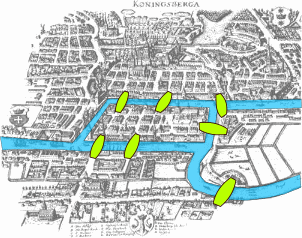
\includegraphics[width=.3\textwidth{}]{Konigsberg_bridges.png}
    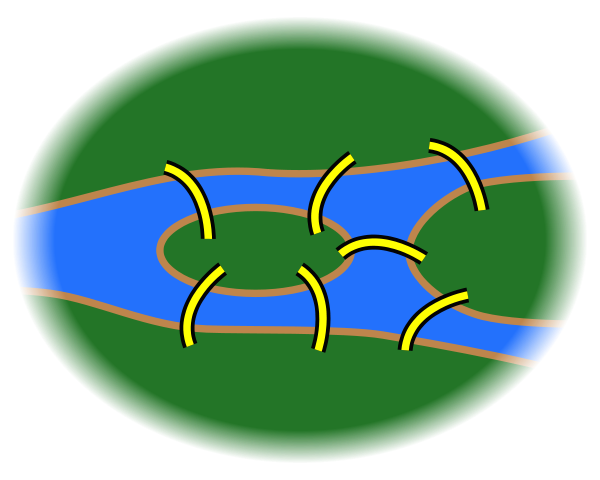
\includegraphics[width=.3\textwidth{}]{600px-7_bridges.svg.png}
    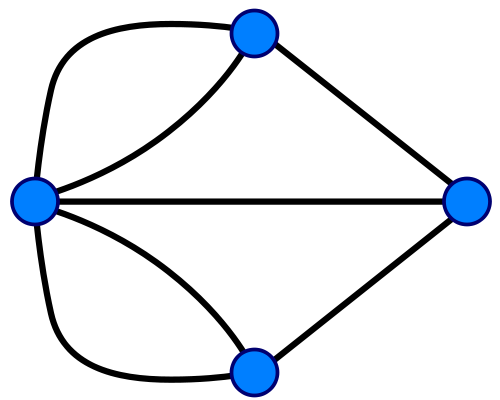
\includegraphics[width=.3\textwidth{}]{500px-Konigsburg_graph.svg.png}
  \end{figure}
  
\end{frame}

\begin{frame}{图的着色问题}
  \begin{block}{}
    给定一张地图,是否可以用四种颜色对其中的区域进行着色,使得任何相邻区域的颜色都不相同
  \end{block}

  \begin{figure}
    \centering
    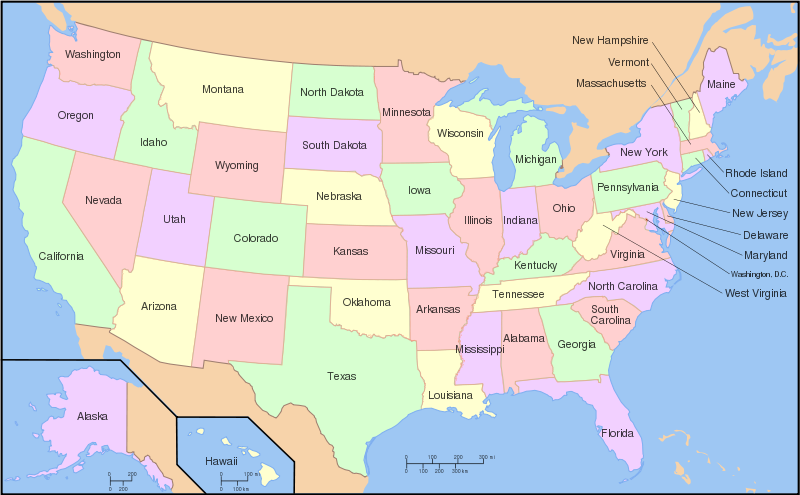
\includegraphics[width=.6\textwidth{}]{Map_of_USA_with_state_names.svg.png}
  \end{figure}
  
\end{frame}

\begin{frame}{图的着色问题}
  \begin{itemize}
  \item 四色定理于1977年由Appel, Haken和Koch证明
  \end{itemize}
  \begin{figure}
    \centering
    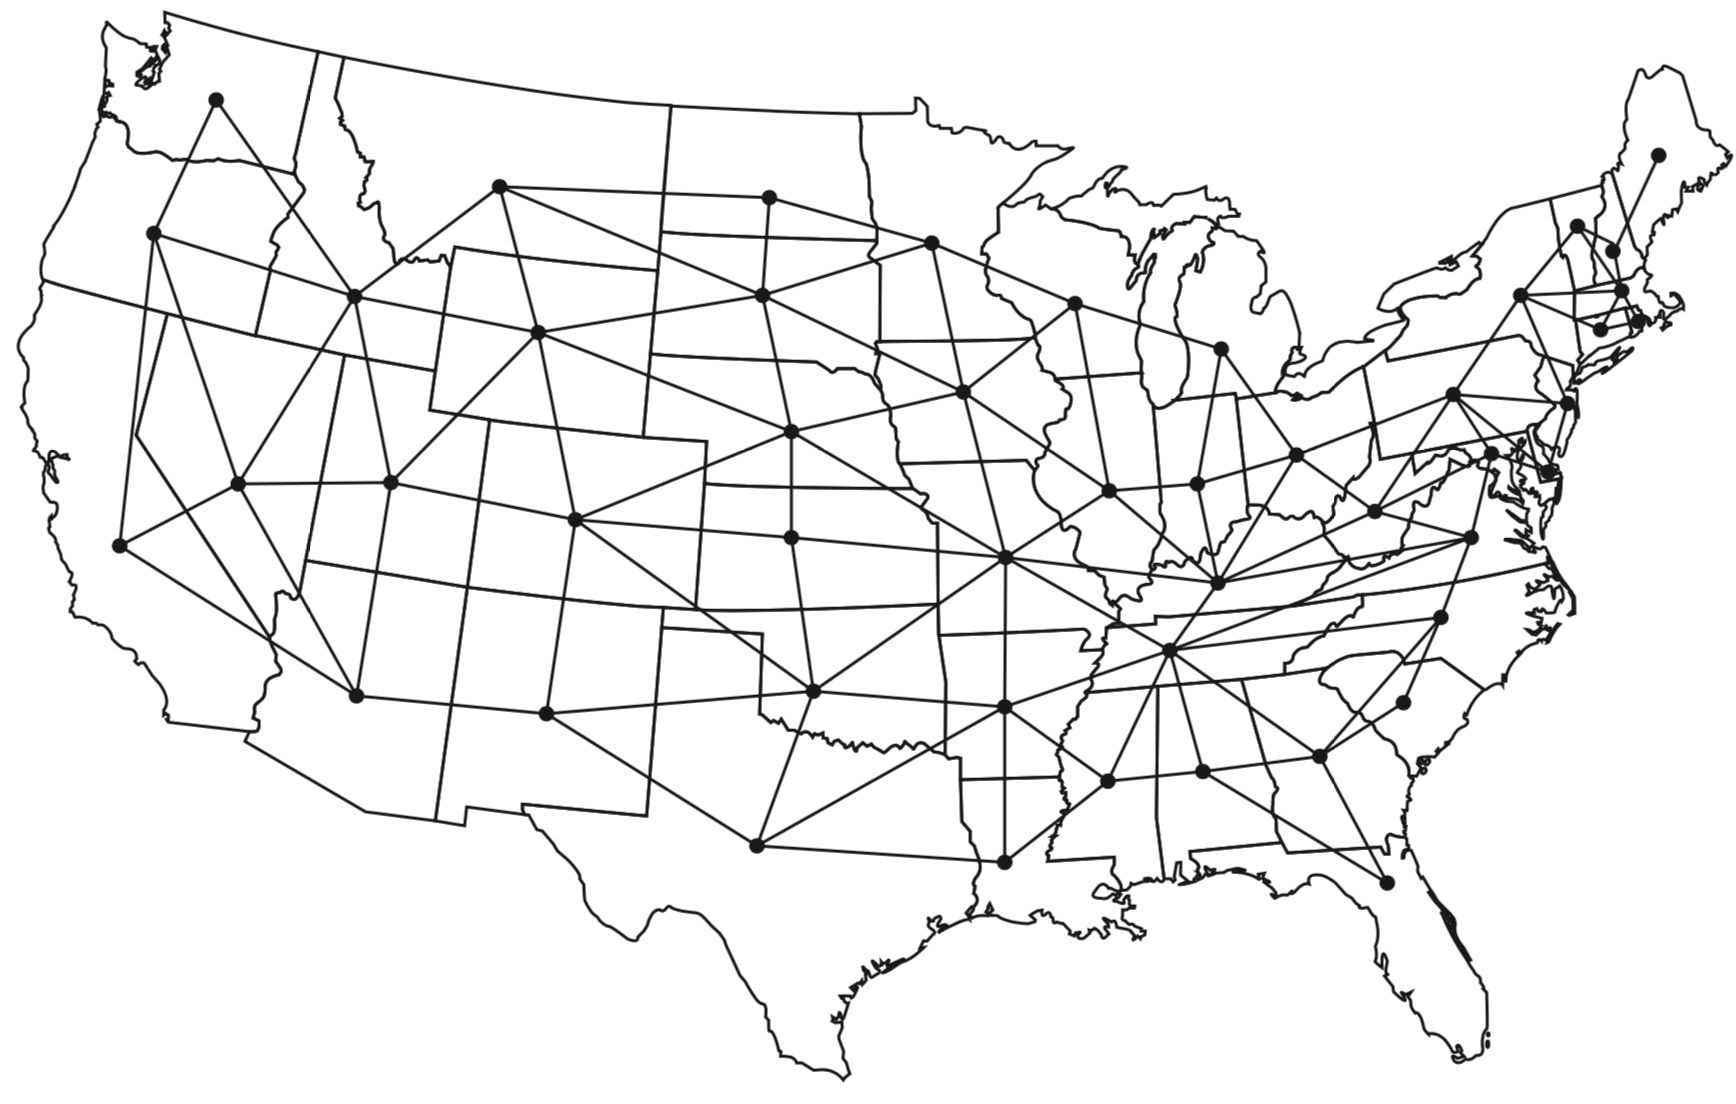
\includegraphics[height=.35\textheight{}]{map_graph2.png}
    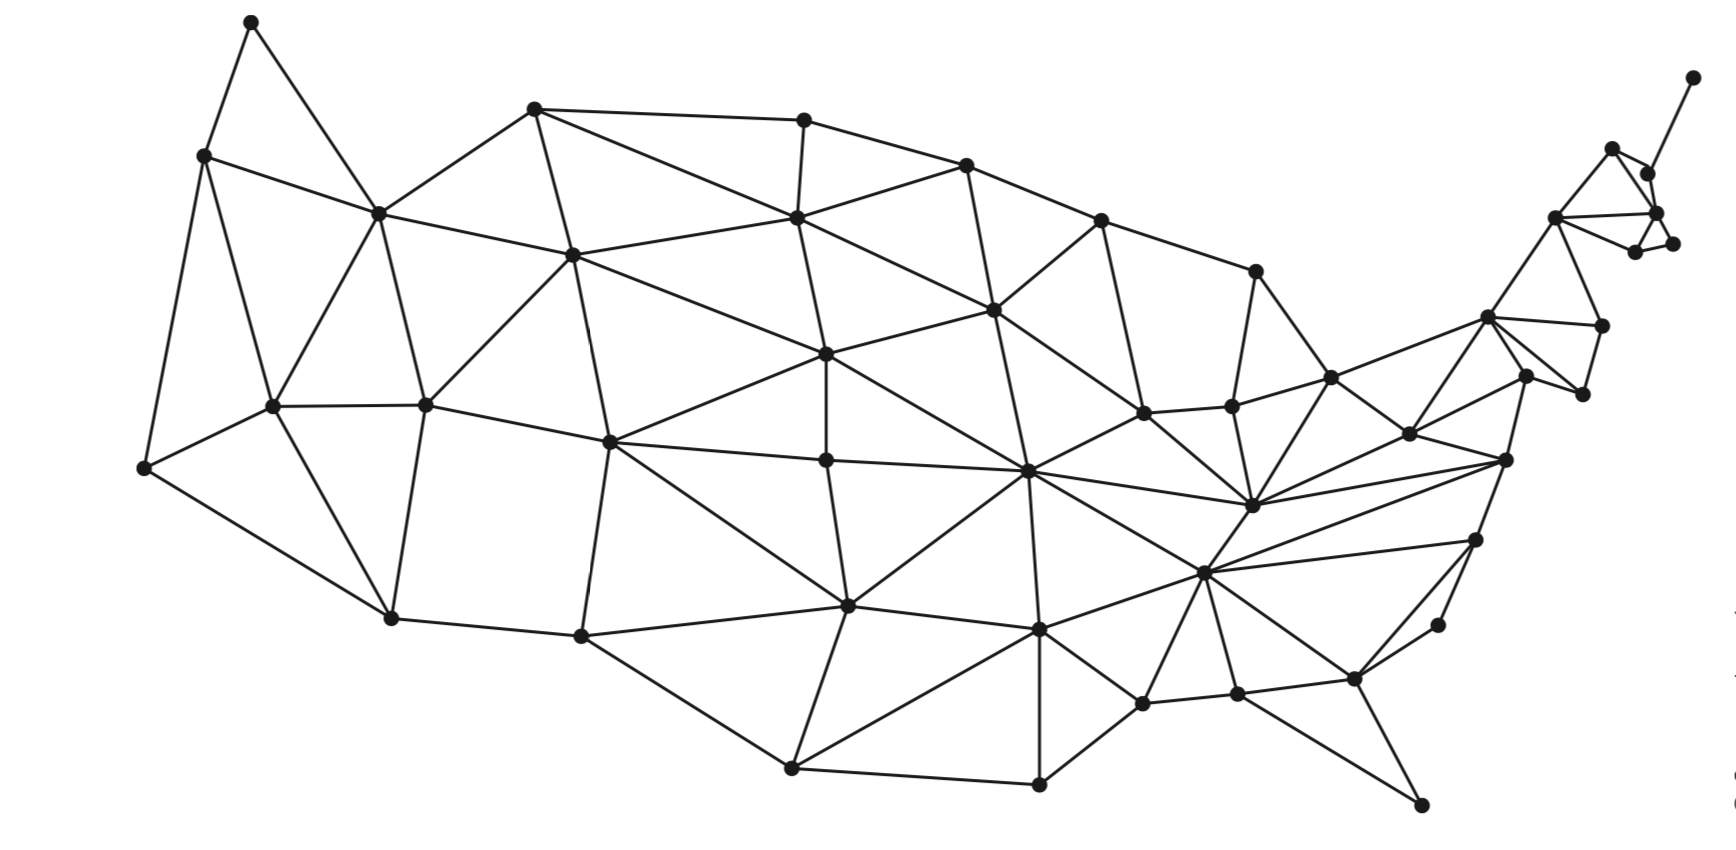
\includegraphics[height=.35\textheight{}]{map_graph.png}
  \end{figure}
  
\end{frame}

\begin{frame}{图着色的应用}
  期末考试安排问题
  \begin{itemize}
  \item 每门课程创建一个顶点
  \item 如果一个学生同时选了某两个顶点对应的课程的话,就在这两个顶点之间画一条边
  \item 对该图进行着色
  \item 学生每种颜色的课程最多只能选一门
  \item 按照课程的颜色安排考试时间
  \end{itemize}
\end{frame}

\begin{frame}{图的描述}
  \begin{itemize}
  \item 顶点集$V(G) = \{a, b, c, d, e, f, g, h, i\}$
  \item 边集$E(G) = \{ac, ad, af, bd, bg, ch, di, ef, ei, fg, gh, hi\}$
  \item 度$deg(a) = 3$
  \end{itemize}

  \begin{figure}
    \centering
    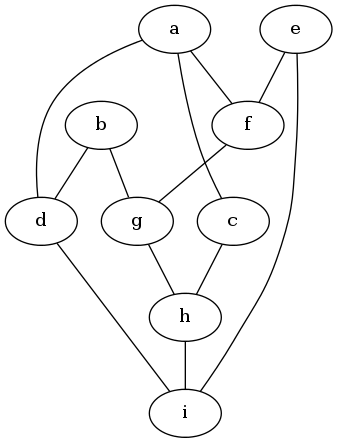
\includegraphics[height=.4\textheight{}]{graph.png}
  \end{figure}
  
\end{frame}

\begin{frame}{Kevin Bacon的六度分隔}

  \begin{figure}
    \begin{minipage}{.2\linewidth}
      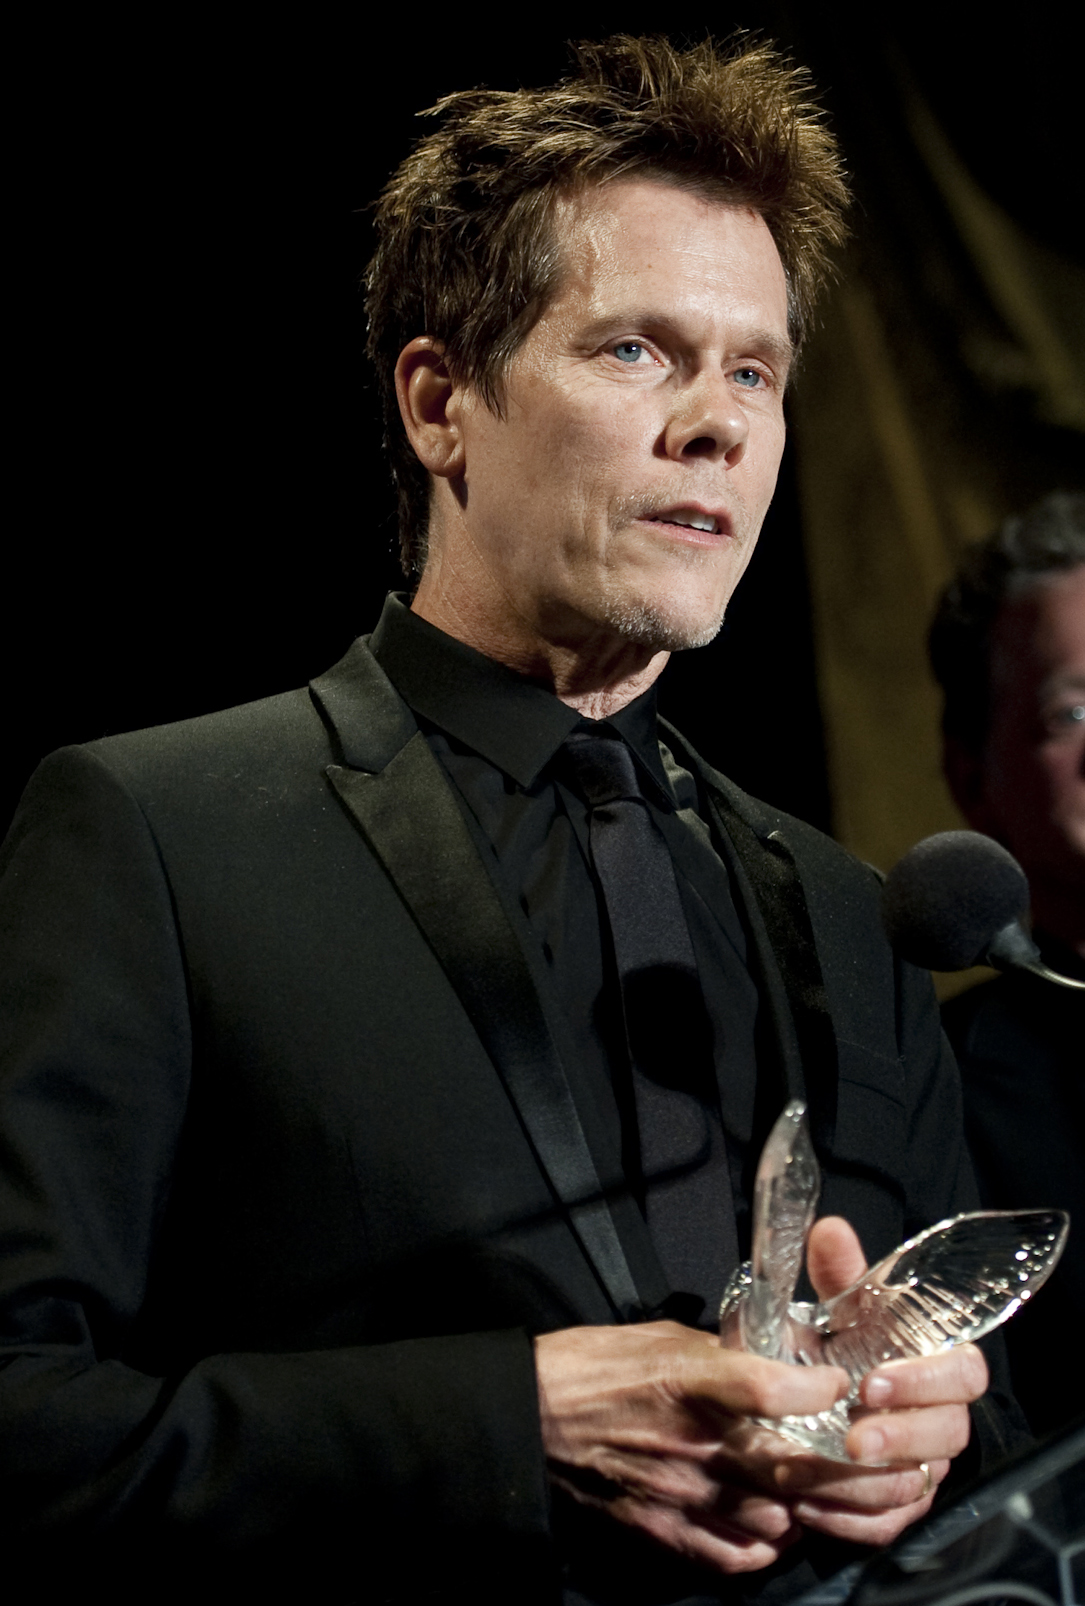
\includegraphics[width=\textwidth]{KevinBaconApr10.jpg}
    \end{minipage}%
    \begin{minipage}{.75\linewidth}
      \begin{itemize}
      \item 将一个演员和Kevin Bacon联系起来所需的最少步数
      \item 类似的还有Erdos数:将一个数学家和Erdos联系起来的最少步骤
      \item Facebook, 人人网
      \item 如何解决?网络科学的新兴研究领域的一部分。
      \end{itemize}
    \end{minipage}
  \end{figure}

\end{frame}

\begin{frame}{用分段线性函数拟合数据}
  \begin{block}{}
    用直线/曲线拟合数据点,必须通过第一点和最后一点
  \end{block}
  \begin{figure}
    \centering
    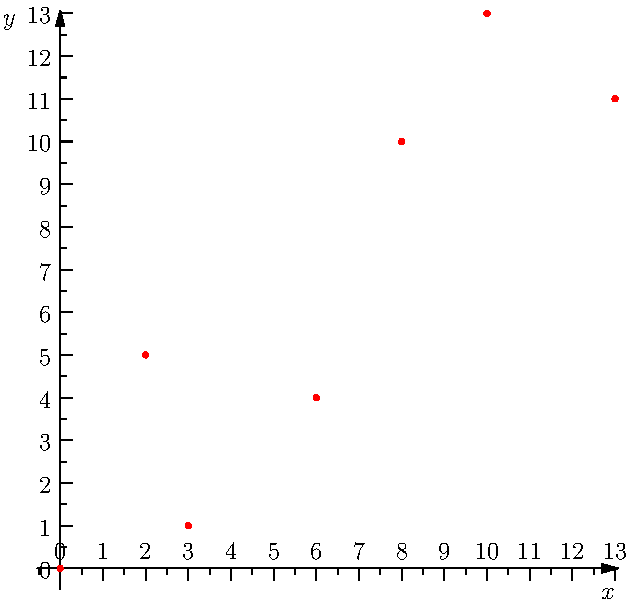
\includegraphics[width=.5\textwidth]{data.pdf}
  \end{figure}
\end{frame}

\begin{frame}{用分段线性函数拟合数据}
  \begin{block}{}
    用一条线段: $y=\frac{y_n-y_1}{x_n-x_1}(x-x_1) + y_1$
  \end{block}
  \begin{figure}
    \centering
    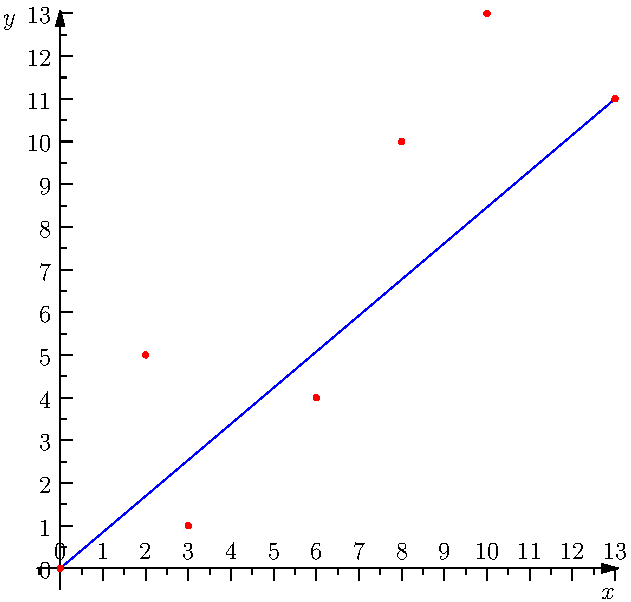
\includegraphics[width=.5\textwidth]{line.pdf}
  \end{figure}
\end{frame}

\begin{frame}{用分段线性函数拟合数据}
  \begin{block}{}
    用多条线段: $y=\frac{y_{i+1}-y_i}{x_{i+1}-x_i}(x-x_i) + y_i, x_i \le x \le x_{i+1}$
  \end{block}
  \begin{figure}
    \centering
    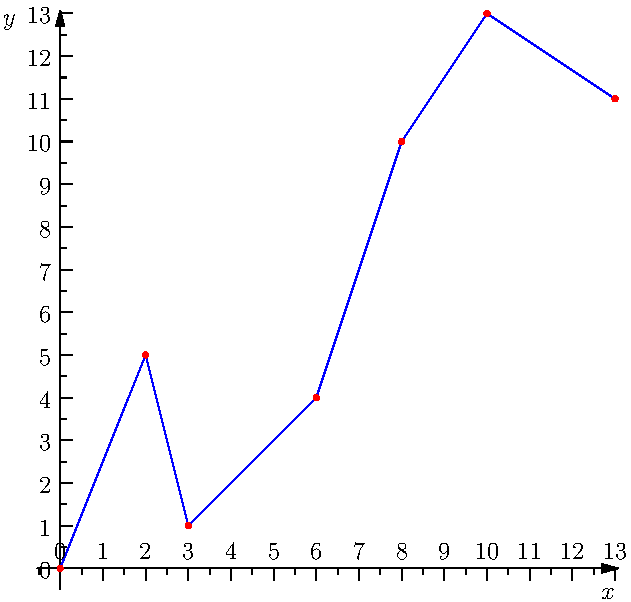
\includegraphics[width=.5\textwidth]{mline.pdf}
  \end{figure}
\end{frame}

\begin{frame}{用分段线性函数拟合数据}
  \begin{block}{}
    折衷方法
  \end{block}
  \begin{figure}
    \centering
    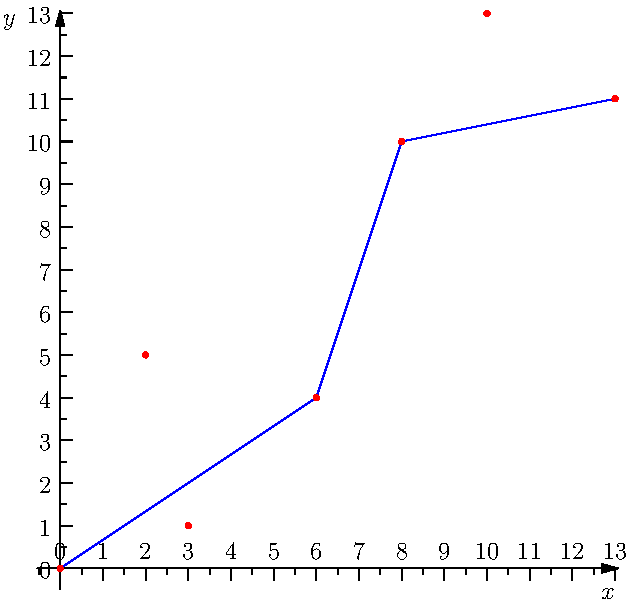
\includegraphics[width=.5\textwidth]{xline.pdf}
  \end{figure}
\end{frame}

\begin{frame}{误差计算}
  \begin{block}{}
    用最小二乘法
  \end{block}
  \begin{table}
    \centering
    \begin{tabular}{c|c|c|c|c}
      \hline
      $k$ & $x_k$ & $f_{1,4}(x_k)$ & $y_k$ & $(f_{1,4}(x_k)-y_k)^2$ \\
      \hline
      1 & 0 & 0 & 0 & 0\\
      \hline
      2 & 2 & $\frac{4}{3}$ & 5 & $\frac{121}{9}$ \\
      \hline
      3 & 3 & 2 & 1 & 1\\
      \hline
      4 & 6 & 4 & 4 & 0\\
      \hline
    \end{tabular}
  \end{table}
\end{frame}

\begin{frame}{考虑线段模型的价格}
  \begin{block}{}
    \[
    \alpha + \beta\sum_{k=1}^4(f_{1,4}(x_k)-y_k)^2
    \]
    令$\alpha=10, \beta=1$, 则:
  \end{block}
  \begin{table}
    \centering
    \begin{tabular}{ccccccc}
      \hline
      & 2 & 3 & 4 & 5 & 6 & 7\\
      \hline
      1 & 10 & 28.7778 & 24.4444 & 36.0625 & 38.77  & 55.503 \\
      2 &  & 10 & 24.0625 & 52.1389 & 61 & 56.9917\\
      3 &  &  & 10 & 15.76 & 14.7755 & 51\\
      4 &  &  &  & 10 & 12.25 & 51\\
      5 &  &  &  & & 10 & 16.76\\
      6 &  &  &  & & & 10\\
      \hline
    \end{tabular}
  \end{table}
\end{frame}

\begin{frame}{如何找出最优线段组合}
  \begin{figure}
    \centering
    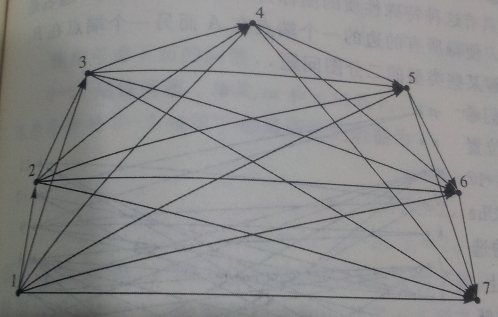
\includegraphics[width=.5\textwidth]{optimal.png}
  \end{figure}

\end{frame}

\begin{frame}{用最短路径求最优组合}
  \begin{figure}
    \centering
    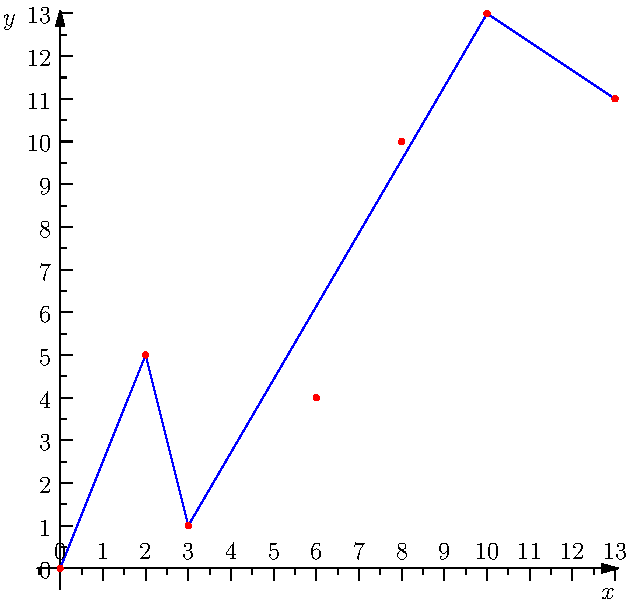
\includegraphics[width=.5\textwidth]{optline.pdf}
  \end{figure}
\end{frame}

\begin{frame}{再论垒球的例子}
  \begin{table}
    \centering
    \begin{tabular}{c|c|c|c|c|c|c|c}
      \hline
      Al & Bo & Che & Doug & Ella & Fay & Gene & Hal\\
      \hline
      2,8 & 1,5,7 & 2,3 & 1,4,5,6,7 & 3,8 & 10,11 & 3,8,11 & 2,4,9\\
      \hline
      Ian & John & Kit & Leo & Moe & Ned & Paul & \\
      \hline
      8,9,10 & 1,5,6,7 & 8,9 & 3,9,11 & 1,4,6,7 && 9,10 &\\
      \hline
    \end{tabular}
  \end{table}
\end{frame}

\begin{frame}{再论垒球的例子}
  \begin{figure}
    \centering
    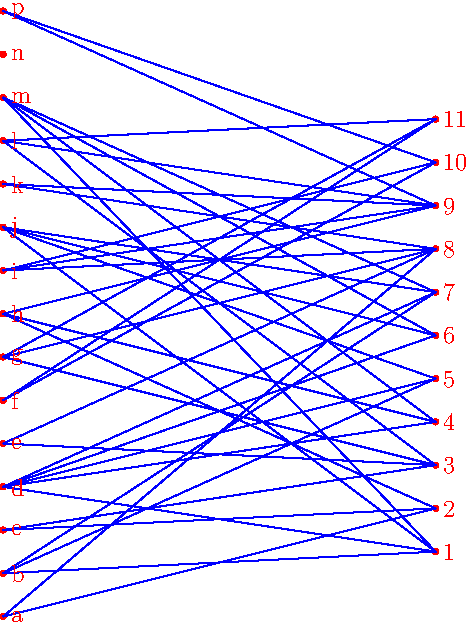
\includegraphics[width=.5\textwidth]{baseball.pdf}
  \end{figure}
\end{frame}

\begin{frame}{最大匹配集}
  \begin{block}{}
    给定任何图$G=(V(G), E(G))$,子集$M \subseteq E(G)$称为匹配集,如果$M$的任何两个成员关于同一个顶点都不是关联的。具有这种性质的边的集合称为是独立的。最大匹配集就是最大可能的匹配。当$G$是两部分为$<A, B>$的二分图时,显然,匹配集的数目不能大于$|A|$也不能大于$|B|$
  \end{block}
\end{frame}

\begin{frame}{$0-1$矩阵问题}
  $m \times n$的$0-1$矩阵
  \[
  \left(\begin{array}{cccccc}
    1 & 0 & 0 & 1 & 1 & 0\\
    1 & 1 & 0 & 0 & 0 & 0\\
    1 & 0 & 1 & 1 & 0 & 0\\
    0 & 1 & 1 & 1 & 0 & 1
  \end{array}\right)
  \]
  \begin{block}{$0-1$矩阵问题}
    给定$m$和$n$以及$r_1, r_2,...,r_m$和$s_1, s_2, ..., s_n$的值,是否存在满足这些条件的$0-1$矩阵?如果$r_1+r_2+...+r_m \neq s_1 + s_2 +...+s_n$呢?
  \end{block}

  \begin{itemize}
  \item $m=4, n=6$
  \item $r_1=3, r_2=2, r_3=3, r_4=4$
  \item $s_1=3, s_2=2, s_3=2, s_4=3, s_5=1, s_6=1$
  \end{itemize}
\end{frame}

\begin{frame}{供应商问题}

  最大流问题

  \begin{figure}
    \centering
    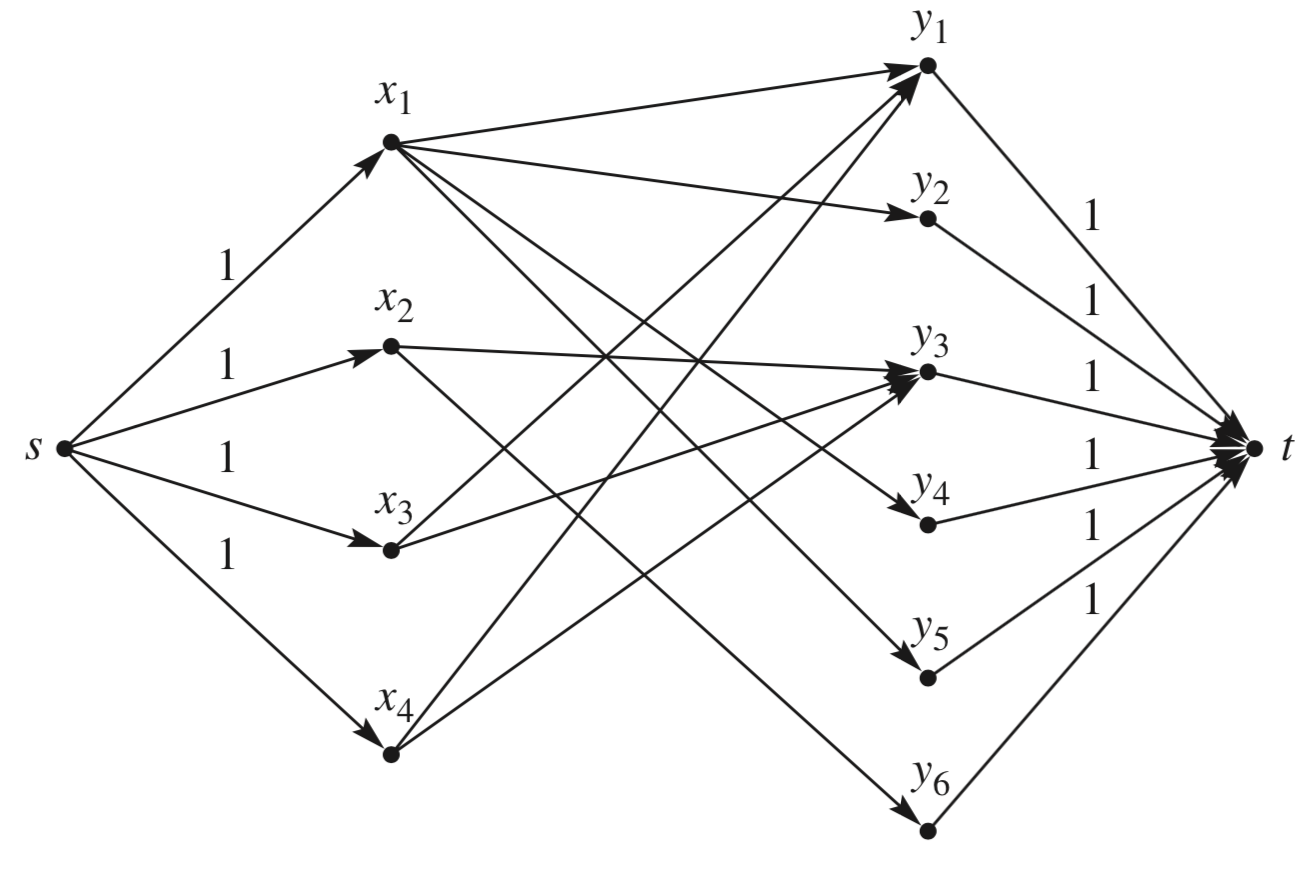
\includegraphics[width=.6\textwidth]{maxflow.png}
  \end{figure}
\end{frame}

\begin{frame}{维护城市治安}
  \begin{figure}
    \centering
    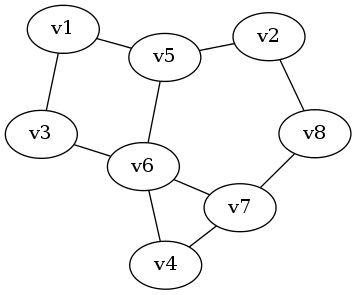
\includegraphics[width=.4\textwidth]{vertexcover.png}
  \end{figure}

  \begin{block}{顶点覆盖问题}
    给定一个图$G=(V(G), E(G))$,顶点覆盖问题就是要寻找一个成员数最少的子集$S \subseteq V(G)$使得图中每条边与$S$中至少一个成员关联。
  \end{block}
  
\end{frame}

\begin{frame}{最短路径算法}
  \begin{itemize}
  \item Dijkstra算法解决了单源的最短路径算法问题
  \item Bellman-Ford算法解决了边权值可负的单源最短路径问题
  \item $A^*$搜索算法用启发式技术加速搜索,找出一对最短路径
  \item Floyd-Warshall算法能够找出图中所有的最短路径
  \item Johnson算法能够找出图中所有的最短路径,对于稀疏图来说速度比Floyd-Warshall算法更快
  \end{itemize}

\end{frame}

\begin{frame}{Dijkstra算法}
  \begin{table}
    \centering
    \begin{tabular}{l|l}
      \rowcolor{lightgray}\textbf{输入} & 图$G=(V(G), E(G))$的源$s$和汇$t$,$ij \in E(G)$的边长$c_{ij} \ge 0$\\
      \textbf{输出} & $G$中$s$到$t$的最短路径的长度\\
      \rowcolor{lightgray}\textbf{第0步} & 从对顶点做标记开始:$L(s) = 0$, 除$s$之外的$L(i)=\infty$,\\
      \textbf{第1步} & 将最小标记的点(若有几个随机取一个)标记为永久标记\\
      \rowcolor{lightgray}\textbf{第2步} & 更新永久标记$i$的邻节点$j$: $L(j) = min\{L(i) + c_{ij}\}$\\
    \end{tabular}
  \end{table}
  \begin{figure}
    \centering
    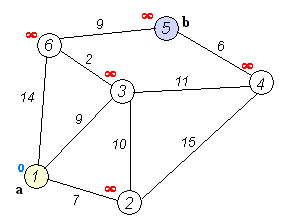
\includegraphics[width=.3\textwidth]{Dijksta_Anim.png}
  \end{figure}
\end{frame}

\begin{frame}{最大流问题}
  \begin{figure}
    \centering
    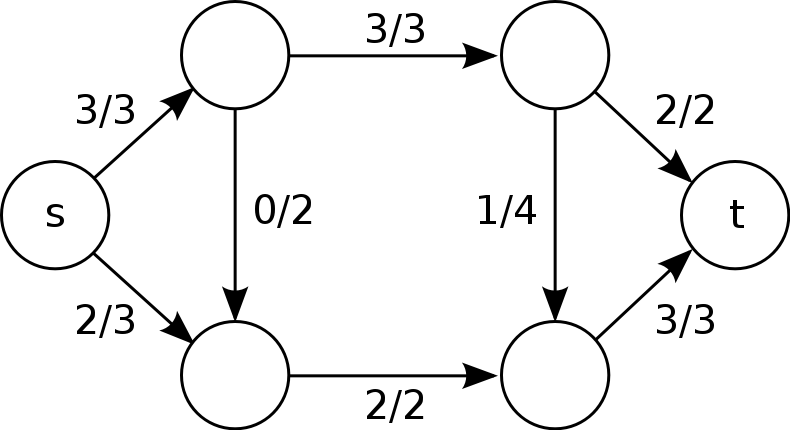
\includegraphics[width=.6\textwidth]{Max_flow.svg.png}
  \end{figure}

  \begin{block}{}
    给定一个有向图$G=(V(G), A(G))$,源$s$和汇$t$,以及对每条有向边$ij \in A(G)$的有限流容量$u_{ij}$,求图中从顶点$s$到顶点$t$的最大流
  \end{block}
  
\end{frame}

\begin{frame}{最大流算法}
  \begin{table}
    \centering
    \begin{tabular}{l|l}
      \rowcolor{lightgray} & 有向图$G=(V(G), A(G))$的源$s$和汇$t$,\\
      \rowcolor{lightgray}\multirow{-2}*\textbf{输入} & 有向边$ij \in A(G)$的容量$u_{ij}$\\
      \textbf{输出} & $G$中从顶点$s$到顶点$t$的最大流\\
      \rowcolor{lightgray}\textbf{第0步} & $f_c \leftarrow 0$\\
      \textbf{第1步} & 从图中找出一条$s$到$t$的有向路径,若没有,停止\\
      \rowcolor{lightgray}\textbf{\quad{}第2步} & 计算$u_{min}$,即有向路径的最小容量\\
      \multirow{2}*{\textbf{\quad{}第3步}} & 对有向路径中的每条有向边$i, j$,\\
      & 更新当前图中的剩余容量$u_{ij} \leftarrow u_{ij}-u_{min}$\\
      \rowcolor{lightgray}\textbf{第5步} & 令$f_c \leftarrow f_c + u_{min}$,回到第1步
    \end{tabular}
  \end{table}
\end{frame}

\begin{frame}{利用最大流求解二分图匹配问题}
  \begin{block}{}
    将匹配问题转化为最大流问题
  \end{block}

  \begin{figure}
    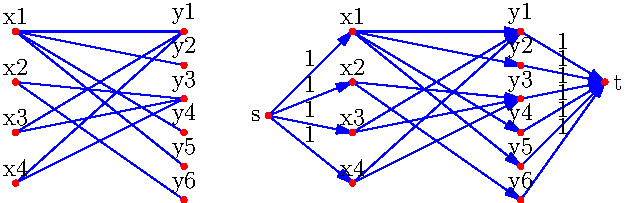
\includegraphics[width=.8\textwidth]{maxmatch-arrow.pdf}
  \end{figure}
\end{frame}

\begin{frame}{旅行商问题}
  \begin{block}{}
    给定一个完全图$G=(V(G), E(G))$,以及$E(G)$中每条边$ij$的费用$c_{ij}$,求最小费用的一条行程。(没有很好的解法)
  \end{block}

  \begin{figure}
    \begin{minipage}{.5\linewidth}
      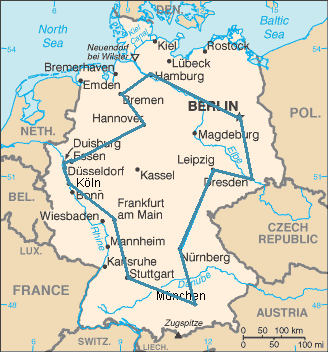
\includegraphics[width=.8\textwidth]{TSP_Deutschland_3.png}
    \end{minipage}%
    \begin{minipage}{.5\linewidth}
      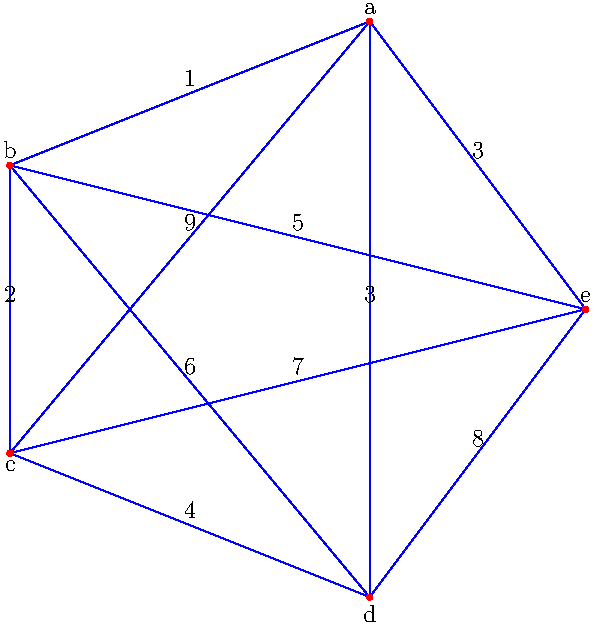
\includegraphics[width=.8\textwidth]{salesman.pdf}
    \end{minipage}
  \end{figure}
  
\end{frame}

\begin{frame}{用数学规划解顶点覆盖问题}
  \begin{figure}
    \centering
    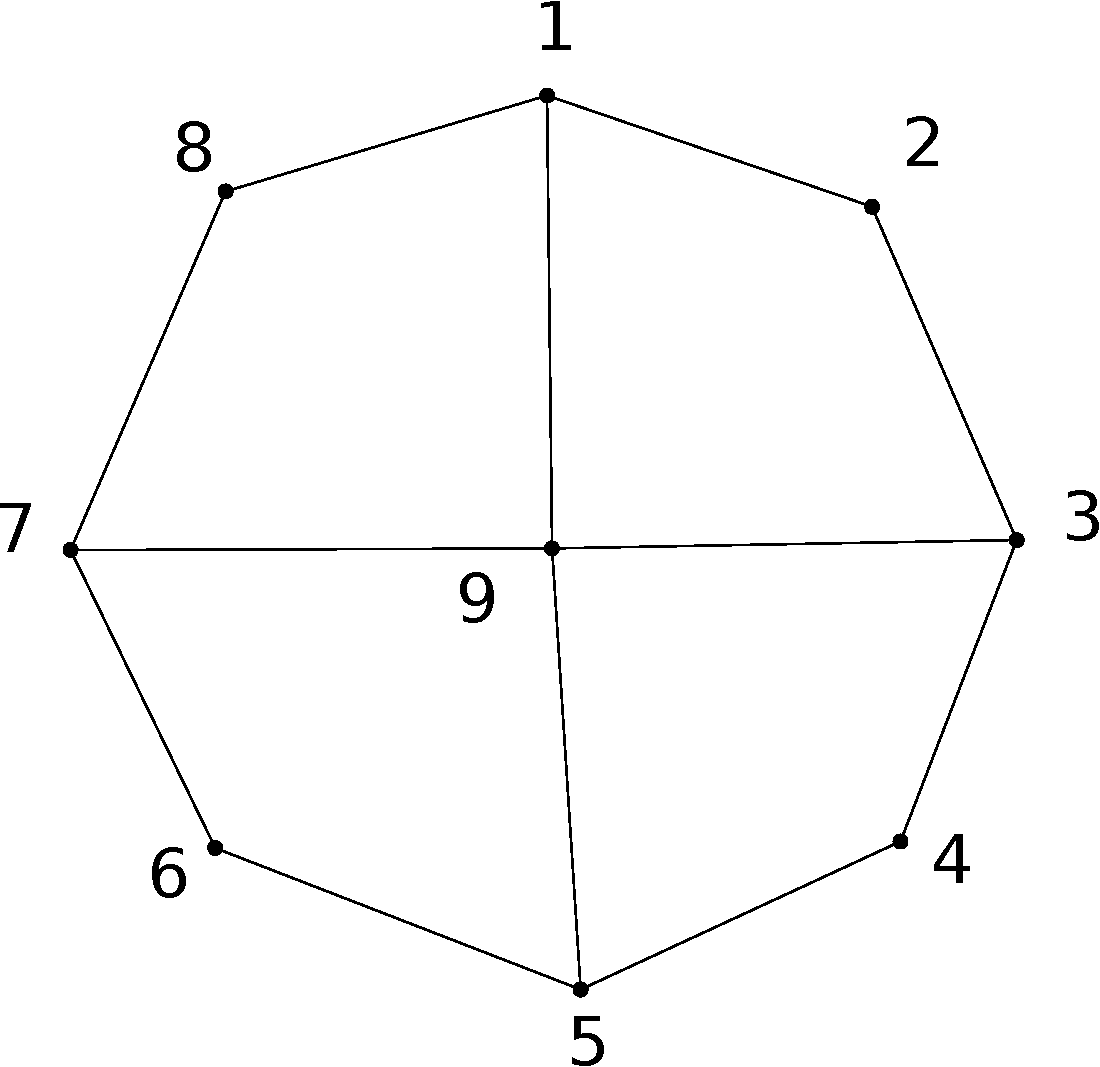
\includegraphics[width=.4\textwidth]{city.pdf}
  \end{figure}
  
  令:
  \[
  x_i =\left\{
  \begin{array}{cc}
    1 & \text{如果} i \in S\\
    0 & \text{如果} i \notin S
  \end{array}
  \right.
  \]
\end{frame}

\begin{frame}{如何表示一条路径被覆盖?}
  \begin{itemize}
  \item<1-> 穷举: 计算量大
  \item<2-> $(1-x_i)(1-x_j) = 0$:非线性
  \item<3-> $x_i+x_j \ge 1$: 线性
  \end{itemize}
\end{frame}

\begin{frame}{顶点覆盖问题的数学规划}
  \[ 
  \begin{array}{lcl}
    & \mbox{Min}\ \sum_{i \in V(G)} x_i & \\
    \mbox{s.t.} & &  \\
    &
    \begin{array}{cc}
      x_i+x_j \ge 1 & \forall ij \in E(G)\\
      x_i \in \{0, 1\} & \forall i \in V(G)
    \end{array}
    &
  \end{array}
  \]

  \begin{itemize}
  \item 这是一个线性规划
  \item 这是一个整数规划
  \item 这是一个0-1规划
  \end{itemize}

\end{frame}

\begin{frame}{最大流}
  令$x_{ij}$表示从顶点$i$到顶点$j$的流.

  \[ 
  \begin{array}{lcl}
    & \mbox{Max}\ z = \sum_{j} x_{sj} & \\
    \mbox{s.t.} & &  \\
    &
    \begin{array}{cc}
      \sum_i x_{ij} = \sum_k x_{jk} & \forall j \in V(G)-\{s, t\}\\
      x_{ij} \le u_{ij} & \forall ij \in A(G)\\
      x_{ij} \ge 0 & \forall ij \in A(G)
    \end{array}
    &
  \end{array}
  \]
  
\end{frame}

\begin{frame}{课后任务}
  \begin{itemize}
  \item 了解图的各种算法
  \item 编程实现最短路径、最大流等算法
  \end{itemize}
\end{frame}

\begin{frame}
  Questions?
  谢谢!
\end{frame}

\end{document}

%%% Local Variables: 
%%% TeX-master: t
%%% TeX-engine: xetex
%%% End: 
